\documentclass[]{article}
\usepackage{lmodern}
\usepackage{amssymb,amsmath}
\usepackage{ifxetex,ifluatex}
\usepackage{fixltx2e} % provides \textsubscript
\ifnum 0\ifxetex 1\fi\ifluatex 1\fi=0 % if pdftex
  \usepackage[T1]{fontenc}
  \usepackage[utf8]{inputenc}
\else % if luatex or xelatex
  \ifxetex
    \usepackage{mathspec}
  \else
    \usepackage{fontspec}
  \fi
  \defaultfontfeatures{Ligatures=TeX,Scale=MatchLowercase}
\fi
% use upquote if available, for straight quotes in verbatim environments
\IfFileExists{upquote.sty}{\usepackage{upquote}}{}
% use microtype if available
\IfFileExists{microtype.sty}{%
\usepackage{microtype}
\UseMicrotypeSet[protrusion]{basicmath} % disable protrusion for tt fonts
}{}
\usepackage[margin=1in]{geometry}
\usepackage{hyperref}
\hypersetup{unicode=true,
            pdftitle={IDZ\_3},
            pdfauthor={Nikita},
            pdfborder={0 0 0},
            breaklinks=true}
\urlstyle{same}  % don't use monospace font for urls
\usepackage{graphicx,grffile}
\makeatletter
\def\maxwidth{\ifdim\Gin@nat@width>\linewidth\linewidth\else\Gin@nat@width\fi}
\def\maxheight{\ifdim\Gin@nat@height>\textheight\textheight\else\Gin@nat@height\fi}
\makeatother
% Scale images if necessary, so that they will not overflow the page
% margins by default, and it is still possible to overwrite the defaults
% using explicit options in \includegraphics[width, height, ...]{}
\setkeys{Gin}{width=\maxwidth,height=\maxheight,keepaspectratio}
\IfFileExists{parskip.sty}{%
\usepackage{parskip}
}{% else
\setlength{\parindent}{0pt}
\setlength{\parskip}{6pt plus 2pt minus 1pt}
}
\setlength{\emergencystretch}{3em}  % prevent overfull lines
\providecommand{\tightlist}{%
  \setlength{\itemsep}{0pt}\setlength{\parskip}{0pt}}
\setcounter{secnumdepth}{0}
% Redefines (sub)paragraphs to behave more like sections
\ifx\paragraph\undefined\else
\let\oldparagraph\paragraph
\renewcommand{\paragraph}[1]{\oldparagraph{#1}\mbox{}}
\fi
\ifx\subparagraph\undefined\else
\let\oldsubparagraph\subparagraph
\renewcommand{\subparagraph}[1]{\oldsubparagraph{#1}\mbox{}}
\fi

%%% Use protect on footnotes to avoid problems with footnotes in titles
\let\rmarkdownfootnote\footnote%
\def\footnote{\protect\rmarkdownfootnote}

%%% Change title format to be more compact
\usepackage{titling}

% Create subtitle command for use in maketitle
\newcommand{\subtitle}[1]{
  \posttitle{
    \begin{center}\large#1\end{center}
    }
}

\setlength{\droptitle}{-2em}
  \title{IDZ\_3}
  \pretitle{\vspace{\droptitle}\centering\huge}
  \posttitle{\par}
  \author{Nikita}
  \preauthor{\centering\large\emph}
  \postauthor{\par}
  \predate{\centering\large\emph}
  \postdate{\par}
  \date{23.03.17}


\begin{document}
\maketitle

{
\setcounter{tocdepth}{2}
\tableofcontents
}
\section{Построение доверительных интервалов.}\label{--.}

\subsection{Доверительные интервалы для параметров нормального
распределения.}\label{-----.}

Постройте выборку длины 1000 из нормального распределения N (μ = -2,σ =
0.25) (параметры выбираете самостоятельно) Для различных уровней
значимости (a = 0.25, a = 0.1, a = 0.05, a = 0.01)

\[f(x)={\tfrac {1}{\sigma {\sqrt {2\pi }}}}\;e^{-{\frac {(x-\mu )^{2}}{2\sigma ^{2}}}}\]

\begin{verbatim}
##    Min. 1st Qu.  Median    Mean 3rd Qu.    Max. 
##   -3.40   -2.31   -2.00   -1.99   -1.67   -0.38
\end{verbatim}

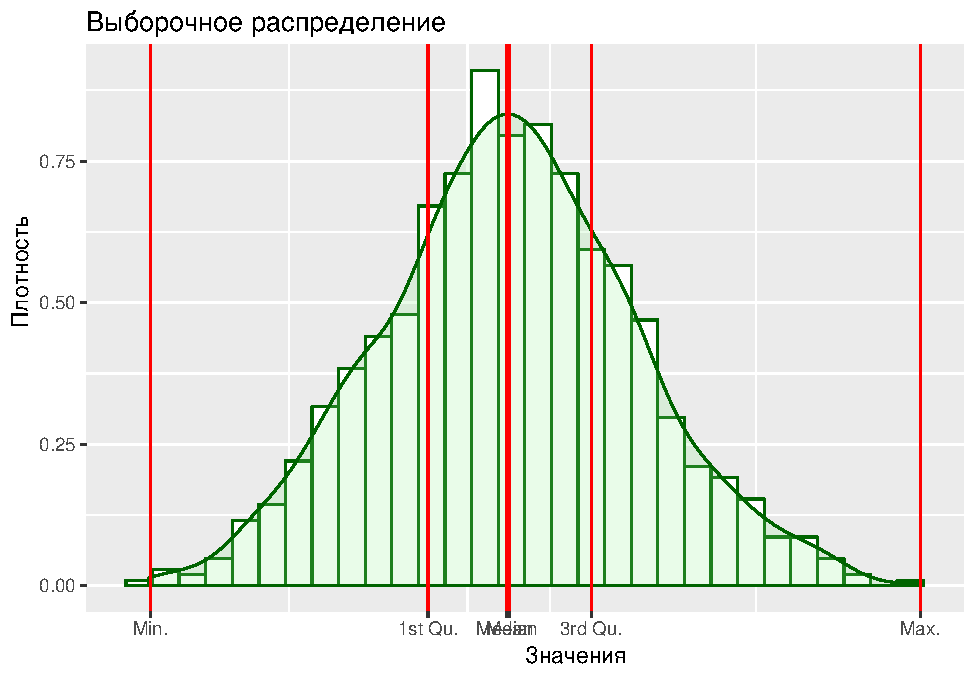
\includegraphics{README_figs/README-graph-1.pdf}

\paragraph{Определение}

Доверительный интервал(\(interval\)) - Интервал, построенный с помощью
случайной выборки из распределения с неизвестным параметром, такой, что
он содержит данный параметр с заданной вероятностью.

Если многократно повторять эксперимент, для каждой выборки рассчитывать
свой доверительный интервал, то в \(p\) случаев истинное среднее будет
находиться внутри доверительного интервала.

т.е. с \((1-a)*100%\) вероятностью мы уверены, что интервал
\(\mu \pm interval\) у выборки включает среднее ГС.

Значения квантилей:

\begin{verbatim}
##      qnorm   qt
## 0.25  1.15 1.15
## 0.1   1.64 1.65
## 0.05  1.96 1.96
## 0.01  2.58 2.58
\end{verbatim}

Чем меньше уровень значимости, тем шире интервал.

\subsubsection{a. Считая дисперсию известной, постройте доверительный
интервал для мат. ожидания.}\label{a.--------.-.}

Пусть \(X_{1},\ldots ,X_{n}\sim \mathrm {N} (\mu ,\sigma ^{2})\) ---
независимая выборка из нормального распределения, где \(\sigma ^{2}\)
--- известная дисперсия. Определим произвольное \(\alpha \in [0,1]\) и
построим доверительный интервал для неизвестного среднего \(\mu\) .

\textbf{Утверждение.} Случайная величина
\(Z={\frac {{\bar {X}}-\mu }{\sigma /{\sqrt {n}}}}\) имеет стандартное
нормальное распределение \(N (0,1)\). Пусть \(z_{\alpha }\) ---
\(\alpha\) -квантиль стандартного нормального распределения. Тогда в
силу симметрии последнего имеем:

\[\mathbb {P} \left(-z_{1-{\frac {\alpha }{2}}}\leq Z\leq z_{1-{\frac {\alpha }{2}}}\right)=1-\alpha\]

После подстановки выражения для \(Z\) и несложных алгебраических
преобразований получаем:

\[ \mathbb {P} \left({\bar {X}}-z_{1-{\frac {\alpha }{2}}}{\frac {\sigma }{\sqrt {n}}}\leq \mu \leq {\bar {X}}+z_{1-{\frac {\alpha }{2}}}{\frac {\sigma }{\sqrt {n}}}\right)=1-\alpha\]
Интервалы:

\begin{verbatim}
##       Left Right
## 0.25 -2.01 -1.97
## 0.1  -2.02 -1.97
## 0.05 -2.02 -1.96
## 0.01 -2.03 -1.95
\end{verbatim}

\subsubsection{b. Считая дисперсию неизвестной, постройте доверительный
интервал для мат. ожидания.}\label{b.--------.-.}

Пусть \(X_{1},\ldots ,X_{n}\sim \mathrm {N} (\mu ,\sigma ^{2})\) ---
независимая выборка из нормального распределения, где
\(\mu ,\sigma ^{2}\) --- неизвестные константы. Построим доверительный
интервал для неизвестного среднего \(\mu\) .

\textbf{Утверждение.} Случайная величина
\(T={\frac {{\bar {X}}-\mu }{S/{\sqrt {n}}}},\) где \(S\) ---
несмещённое выборочное стандартное отклонение, имеет распределение
Стьюдента с \(n-1\) степенями свободы \(t(n-1)\). Пусть
\({\displaystyle t_{\alpha ,n-1}}\) - \({\displaystyle \alpha }\)
квантили распределения Стьюдента. Тогда в силу симметрии последнего
имеем:

\[\mathbb {P} \left(-t_{1-{\frac {\alpha }{2}},n-1}\leq T\leq t_{1-{\frac {\alpha }{2}},n-1}\right)=1-\alpha \]
После подстановки выражения для \(T\) и несложных алгебраических
преобразований получаем:

\[\mathbb {P} \left({\bar {X}}-t_{1-{\frac {\alpha }{2}},n-1}{\frac {S}{\sqrt {n}}}\leq \mu \leq {\bar {X}}+t_{1-{\frac {\alpha }{2}},n-1}{\frac {S}{\sqrt {n}}}\right)=1-\alpha\]
Интервалы:

\begin{verbatim}
##       Left Right
## 0.25 -2.01 -1.97
## 0.1  -2.02 -1.97
## 0.05 -2.02 -1.96
## 0.01 -2.03 -1.95
\end{verbatim}

\subsubsection{c. Постройте доверительный интервал для
дисперсии.}\label{c.-----.}

Пусть \(X_{1},\ldots ,X_{n}\sim {\mathcal {N}}(\mu ,\sigma ^{2})\) ---
независимая выборка из нормального распределения, где \(\mu\) ,
\(\sigma ^{2}\) --- неизвестные константы. Построим доверительный
интервал для неизвестной дисперсии \(\sigma ^{2}\).

Теорема Фишера для нормальных выборок. Случайная величина

\[H={\frac {(n-1)S^{2}}{\sigma ^{2}}},\] где \(S^{2}\) --- несмещённая
выборочная дисперсия, имеет распределение \(\chi ^{2}(n-1)\). Тогда
имеем:

\[ \mathbb {P} \left(\chi _{{\frac {1-\alpha }{2}},n-1}^{2}\leqslant H\leqslant \chi _{{\frac {1+\alpha }{2}},n-1}^{2}\right)=\alpha\]

После подстановки выражения для \(H\) и несложных алгебраических
преобразований получаем:

\[ \mathbb {P} \left({\frac {(n-1)S^{2}}{\chi _{{\frac {1+\alpha }{2}},n-1}^{2}}}\leqslant \sigma ^{2}\leqslant {\frac {(n-1)S^{2}}{\chi _{{\frac {1-\alpha }{2}},n-1}^{2}}}\right)=\alpha\]

\begin{verbatim}
##       Left Right
## 0.25 0.238 0.264
## 0.1  0.233 0.270
## 0.05 0.230 0.274
## 0.01 0.224 0.282
\end{verbatim}

\subsubsection{d. Считая дисперсию s известной, постройте
асимптотический доверительный интервал для a на базе ОМП. Сравните с
результатом пункта a).}\label{d.---s-------a---.-----a.}

Если эксперимент регулярный, то ОМП \(\bar θ_n\) параметра \(θ\)
является

асимптотически нормальной и состоятельной, то есть
\(\sqrt{I(θ)}(\bar θ_n − θ)⇒ N(0,1)\), где \(I(θ)\) --- информация
Фишера для параметра \(θ\) по наблюдениям \(X\).

Можно выбрать квантили \(x_α\), решая уравнение
\(Ф(x_α) = 1- \frac {α}{2}\), где \(Ф\) --- функция распределения
стандартного нормального закона.

В этом случае, в общем виде для параметра \(θ\) доверительный интервал
уровня \(1-α\) будет выглядеть так:

\[[ θ_n − I( θ_n)^{−1 /2} x_{\alpha} , θ_n + I( θ_n)^{−1 /2} x_{\alpha}]\]
Информация Фишера обладает свойством: если имеется выборка из \(n\)

элементов, где \(I_i(θ)\) --- информация Фишера для одного \(i\)-го
элемента выборки,

то \(I(θ)=nI_i(θ)\).\(I(a) = σ^{−2}\) На основании этого свойства и вида
доверительного интервала

построим асимптотический доверительный интервал для среднего:
\[[X−\frac {(sx_α)}{\sqrt n}, X+\frac {(sx_α)}{\sqrt n} ]\]

\begin{verbatim}
##       Left Right
## 0.25 -2.01 -1.97
## 0.1  -2.02 -1.97
## 0.05 -2.02 -1.96
## 0.01 -2.03 -1.95
\end{verbatim}

\subsubsection{e. Считая мат. ожид. а известным, постройте
асимптотический доверительный интервал для s на базе ОМП. Сравните с
результатом пункта c).}\label{e.--.-.--------s---.-----c.}

Если эксперимент регулярный, то ОМП \(\bar θ_n\) параметра \(θ\)
является

асимптотически нормальной и состоятельной, то есть
\(\sqrt{I(θ)}(\bar θ_n − θ)⇒ N(0,1)\), где \(I(θ)\) --- информация
Фишера для параметра \(θ\) по наблюдениям \(X\).

Можно выбрать квантили \(x_α\), решая уравнение
\(Ф(x_α) = 1- \frac {α}{2}\), где \(Ф\) --- функция распределения
стандартного нормального закона.

В этом случае, в общем виде для параметра \(θ\) доверительный интервал
уровня \(1-α\) будет выглядеть так:

\[[ θ_n − I( θ_n)^{−1 /2} x_{\alpha} , θ_n + I( θ_n)^{−1 /2} x_{\alpha}]\]
Информация Фишера обладает свойством: если имеется выборка из \(n\)

элементов, где \(I_i(θ)\) --- информация Фишера для одного \(i\)-го
элемента выборки,

то \(I(θ)=nI_i(θ)\).\(I(σ^2) = σ^{−4/2}\) На основании этого свойства и
вида доверительного интервала

построим асимптотический доверительный интервал для дисперсии:

\[[s^2−\sqrt \frac {2}{n} s^2 x_\alpha, s^2+\sqrt \frac {2}{n} s^2 x_\alpha]\]

\begin{verbatim}
##       Left Right
## 0.25 0.233 0.259
## 0.1  0.228 0.264
## 0.05 0.224 0.267
## 0.01 0.218 0.274
\end{verbatim}

\subsubsection{Сравнение E c C}\label{-e-c-c}

\begin{verbatim}
##      E.minus.C
## 0.25   0.00474
## 0.1    0.00507
## 0.05   0.00536
## 0.01   0.00609
\end{verbatim}

Как видим значимых отличий нет.

\subsubsection{Сравнение D c A}\label{-d-c-a}

\begin{verbatim}
##      D.minus.A
## 0.25         0
## 0.1          0
## 0.05         0
## 0.01         0
\end{verbatim}

Как видим значимых отличий нет.

То же видим на графике
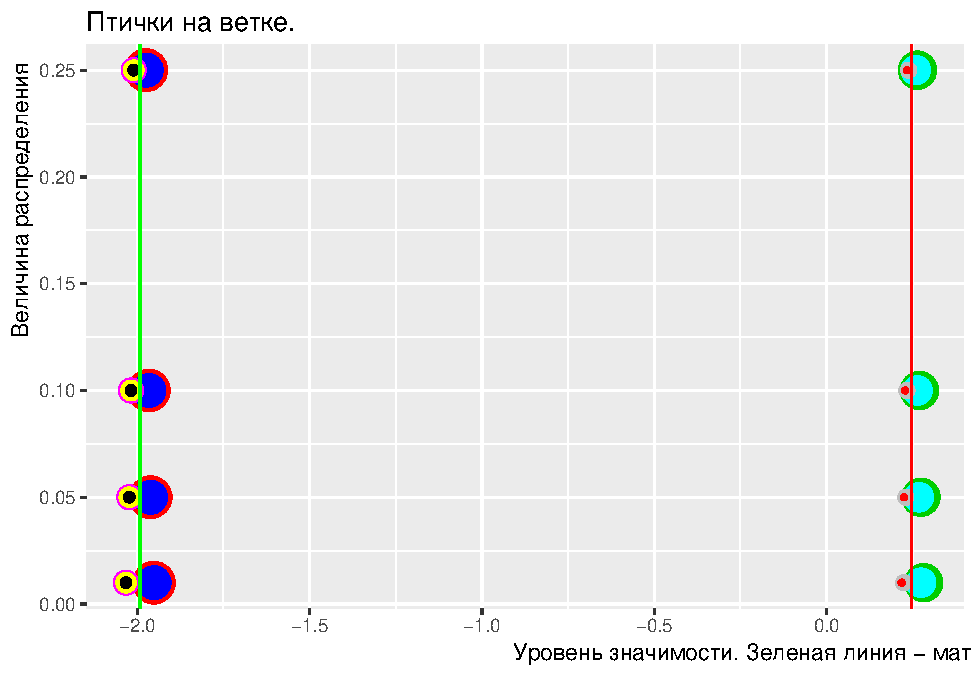
\includegraphics{README_figs/README-unnamed-chunk-10-1.pdf}

\subsection{Асимптотические доверительные интервалы на базе
ОМП}\label{-----}

На основании оценок, полученных в предыдущем ДЗ (задания 2 и 3),
постройте асимптотические доверительные интервалы уровней значимости(a =
0.25, a = 0.1, a = 0.05, a = 0.01).

Я еще не доделал то идз, чтобы сделать эту часть))


\end{document}
